%%%%%%%%%%%%%%%%%%%%%%%%%%%%%%%%%%%%%%%%%%%%%%%%%%%%%%%%%%%%%%%%%%%%%%%%%%%%%%

\documentclass{l3deliverable}

%%%%%%%%%%%%%%%%%%%%%%%%%%%%%%%%%%%%%%%%%%%%%%%%%%%%%%%%%%%%%%%%%%%%%%%%%%%%%%

\usepackage{graphicx}%
%

\version{Reviewed -- 28/11/2012 by Team W

Draft version -- 31/10/2012 by Team W}

\usepackage{tabularx}%
\usepackage{url}%
\usepackage{usecasedescription}%

%%%%%%%%%%%%%%%%%%%%%%%%%%%%%%%%%%%%%%%%%%%%%%%%%%%%%%%%%%%%%%%%%%%%%%%%%%%%%%
%% Check these macro values for appropriateness for your own document.

\title{Requirements Document}

\author{
    Gordon Reid: 1002536R\\
    Ryan Wells: 1002253W\\
    Kristopher Stewart: 1007175S\\
    David Selkirk: 1003646S\\
    James Gallagher: 0800899G\\
}

\date{29 November 2012}

\deliverableID{D3}
\project{PSD3 GE1 - Internship Management System}
\team{W}

%%%%%%%%%%%%%%%%%%%%%%%%%%%%%%%%%%%%%%%%%%%%%%%%%%%%%%%%%%%%%%%%%%%%%%%%%%%%%%

\begin{document}

%%%%%%%%%%%%%%%%%%%%%%%%%%%%%%%%%%%%%%%%%%%%%%%%%%%%%%%%%%%%%%%%%%%%%%%%%%%%%%

\maketitle

\tableofcontents

\newpage

%%%%%%%%%%%%%%%%%%%%%%%%%%%%%%%%%%%%%%%%%%%%%%%%%%%%%%%%%%%%%%%%%%%%%%%%%%%%%%
%% Standard section for all documents

\section{Introduction}

\subsection{Identification}

This is the requirements specification for the Level 3 project by Team W. The
project is based on an internship management system for Software Engineering
(SE), and Electronic and Software Engineering (ESE) students, studying in the
School of Computing Science.

\subsection{Related Documentation}

PSD3 Group Exercise Description:

\url{fims.moodle.gla.ac.uk/file.php/128/coursework/psd3-ge-1-rev3278.pdf}

\subsection{Purpose and Description of Document}

This document proposes a description of the behaviour of the
internship management system as proposed by Team W. The document gives a
clear overview of the main functions that the School of Computing
Science Internship Management system must possess, established by our finidings through the requirements gathering process. \\

This document will endeavour to clarify the requirements of the system in a detailed and concise manner through the following methods: detailed system and actor descriptions, domain modelling, use case descriptions with diagrams, and non functional requirements of the system.

\subsection{Document Status and Schedule}

The creation of this document was aided by two previous Professional Software
Development coursework deliverables, a client interview with course
lecturer Rose English, and a stakeholder panel with four main stakeholders.
This document has undergone two draft stages and this is the reviewed copy. This document is still subject to change if and when requirements change.

%%%%%%%%%%%%%%%%%%%%%%%%%%%%%%%%%%%%%%%%%%%%%%%%%%%%%%%%%%%%%%%%%%%%%%%%%%%%%%

\section{Extended Problem Definition}

%%%%%%%%%%%%%%%%%%%%%%%%%%%%%%%%%%%%%%%%%%%%%%%%%%%%%%%%%%%%%%%%%%%%%%%%%%%%%%

The School of Computing Science at the University of Glasgow are looking for a unified system for 
collecting, reviewing, and publishing internship advertisements. Stated features features which the system must possess include: 
\begin{itemize}
\item Submission of internship advertisements,
\item Review, comment, and publication of internship advertisements,
\item Viewing of internship advertisements, and
\item Notification of successful internship applications.
\end{itemize}
The system does not have to support the application process, this is outsite the scope of the system and students are to use the companies own processes for this. \\ \\ 
These sections are extrapolated below with further information gathered from interviews and panelists.

\subsection{Submission of internship advertisements}
Companies wishing to submit advertisements to the system are required to first
contact the course coordinator for access to the system and a system login will be given to a legitimate company. This ensures validity of submissions.
\\ \\
Only textual data can be submitted as part of an advertisement. A company must fill specific fields for the advertisement to be submitted, these fields have not been formalised but are assumidly: what the internship entails, salary, name and location of company and internship manager and contact details.
\\ \\
A further check may be to ensure no duplicate entries to the system, but may be redundant as the Course Coordinator must approve each advertisement before it becomes live on the system.

\subsection{Review, comment, and publication of internship advertisements}
Each advertisement has to be reviewed and accepted by the course coordinator
prior to becoming live on the system for students to view. As part of the review process, the
course coordinator can accept or reject the advertisement. In the event of an application being rejected, the system is not required to submit feedback to the company, this is outside the scope of the system and is handled seperately
by the course coordinator.
\\ \\
The Course Coordinator is required to state whether or not a given placement is suitable for Software Engineering or Electronic and Software Engineering students.
\\ \\
When an internship advertisement has been reviewed and published, students 
are to be notified. This can be done either by mass email or via a 
notification presented to the user on login to the system.
\\ \\
It was noted that a Course Coordinator should have an overview `Dashboard' on the system where they can quickly see how many advertisements are live, pending and rejected, and also how many students have confirmed internships, are pending confirmation of internships through the Course Coordinator, have applied for internships and have not applied for internships thus far.

\subsection{Viewing of internshop advertisements}
The system is available for all Computing Science students to access and 
all Computing Science students can apply for any internship available, however SE/ESE students
are required to apply for SE/ESE suitable internships.
\\ \\
The login process will be linked with existing student accounts and be
handled separately to the system and thus is outside the scope of the system. However care and consideration concerning how and where this will be integrated is good software practice and will make the system more maintainable.

\subsection{Notification of successful internship applications}
Students will have a status to allow the course coordinator to track progress
through the system. A student can have the status of: Confirmed an internship, pending
approval to an internship success, awaiting response to an internship application, or yet to apply/no current 
application in progress. The student will be able to notify the Course Coordinator of a successful placement through the system and this process will be able to convey the necessary information, which is assumidly the details of the advertisement.

%%%%%%%%%%%%%%%%%%%%%%%%%%%%%%%%%%%%%%%%%%%%%%%%%%%%%%%%%%%%%%%%%%%%%%%%%%%%%%

\section{System Scope}

%Give an overview of the system here, in the context of the surrounding
%environment.  Use case diagrams can be used to illustrate the
%interactions between actors in the environment and the system.

%You should explain the assumptions you have made in defining the
%boundary of the system (i.e. what the system will and will not do).

%Describe any conflicts in requirements expressed by different
%stakeholders, how you resolved them and why.

The system is to be a unified system of gathering, approving and viewing internships that are relevant to Third Year Computing Science, Software and Electronic and Software Engineers.
\\ \\
The system  must allow companies to submit advertisements 
of internships and upon approval by the course coordinator the 
advertisements can be viewed by students. The students with successful applications can then notify 
the coordinator, who can approve or deny the students internship based on 
course outlines. The system will notify all students of newly available internships.

The system will not provide an application for handling applications. This is outside the scope of the system. Confusion arose when conflicting panelists views were stated on this issue, a distinct contradiction was drawn that the system was to have and was not to have this feature. It was later clarified that the system was not to have this feature. The system will not have any direct contact with a company. This was finalised by panelists.
\\\\
A Company can log in and submit advertisements to the system. They may 
view only their own advertisements, as well as the standardised template for 
advertisements.

A company cannot edit an application after it has gone live. This was a stated requirement that all stakeholders agreed upon. 
\\\\
The Course Coordinator can log in, approve or reject submitted advertisements and can tag advertisements for SE/ESE students only. They can also view and change each students application status, as well as sending 
the student a notification of success reply.

The Course Coordinator cannot edit a pending application. The notification of success reply contains no comments about the reply, this is outside the scope of the system. 
\\\\
The Student may log in and view advertisements. They can send a notification of successful application to an internship, whether it's a job in the system or externally sourced. If the student is a SE/ESE student then the Course Coordinator must review the internship at this stage if it is an externally sourced internship.

%%%%%%%%%%%%%%%%%%%%%%%%%%%%%%%%%%%%%%%%%%%%%%%%%%%%%%%%%%%%%%%%%%%%%%%%%%%%%%

\subsection{System Actors}
\begin{itemize}
\item The Company:

This includes any organisation that wishes to submit 
advertisements to the system. Organisations such as Club21, which handle
many different companies and advertisements, still count as a single Company
with regards to the system.

\item The Course Coordinator: 

This refers to the designated staff member whose responsibility
it is to manage SE internships. This is a single person role, but can be 
passed from one staff member to another in extreme circumstances.

\item The Student: 

This refers to Third Year Students studying under the School of Computing Science at the University of Glasgow.
\end{itemize}
%%%%%%%%%%%%%%%%%%%%%%%%%%%%%%%%%%%%%%%%%%%%%%%%%%%%%%%%%%%%%%%%%%%%%%%%%%%%%%

\subsection{Domain Model}

%Note:this section is giving me trouble, need a plugin to do a visual
%domain model? And just the domain in general is proving difficult to design.

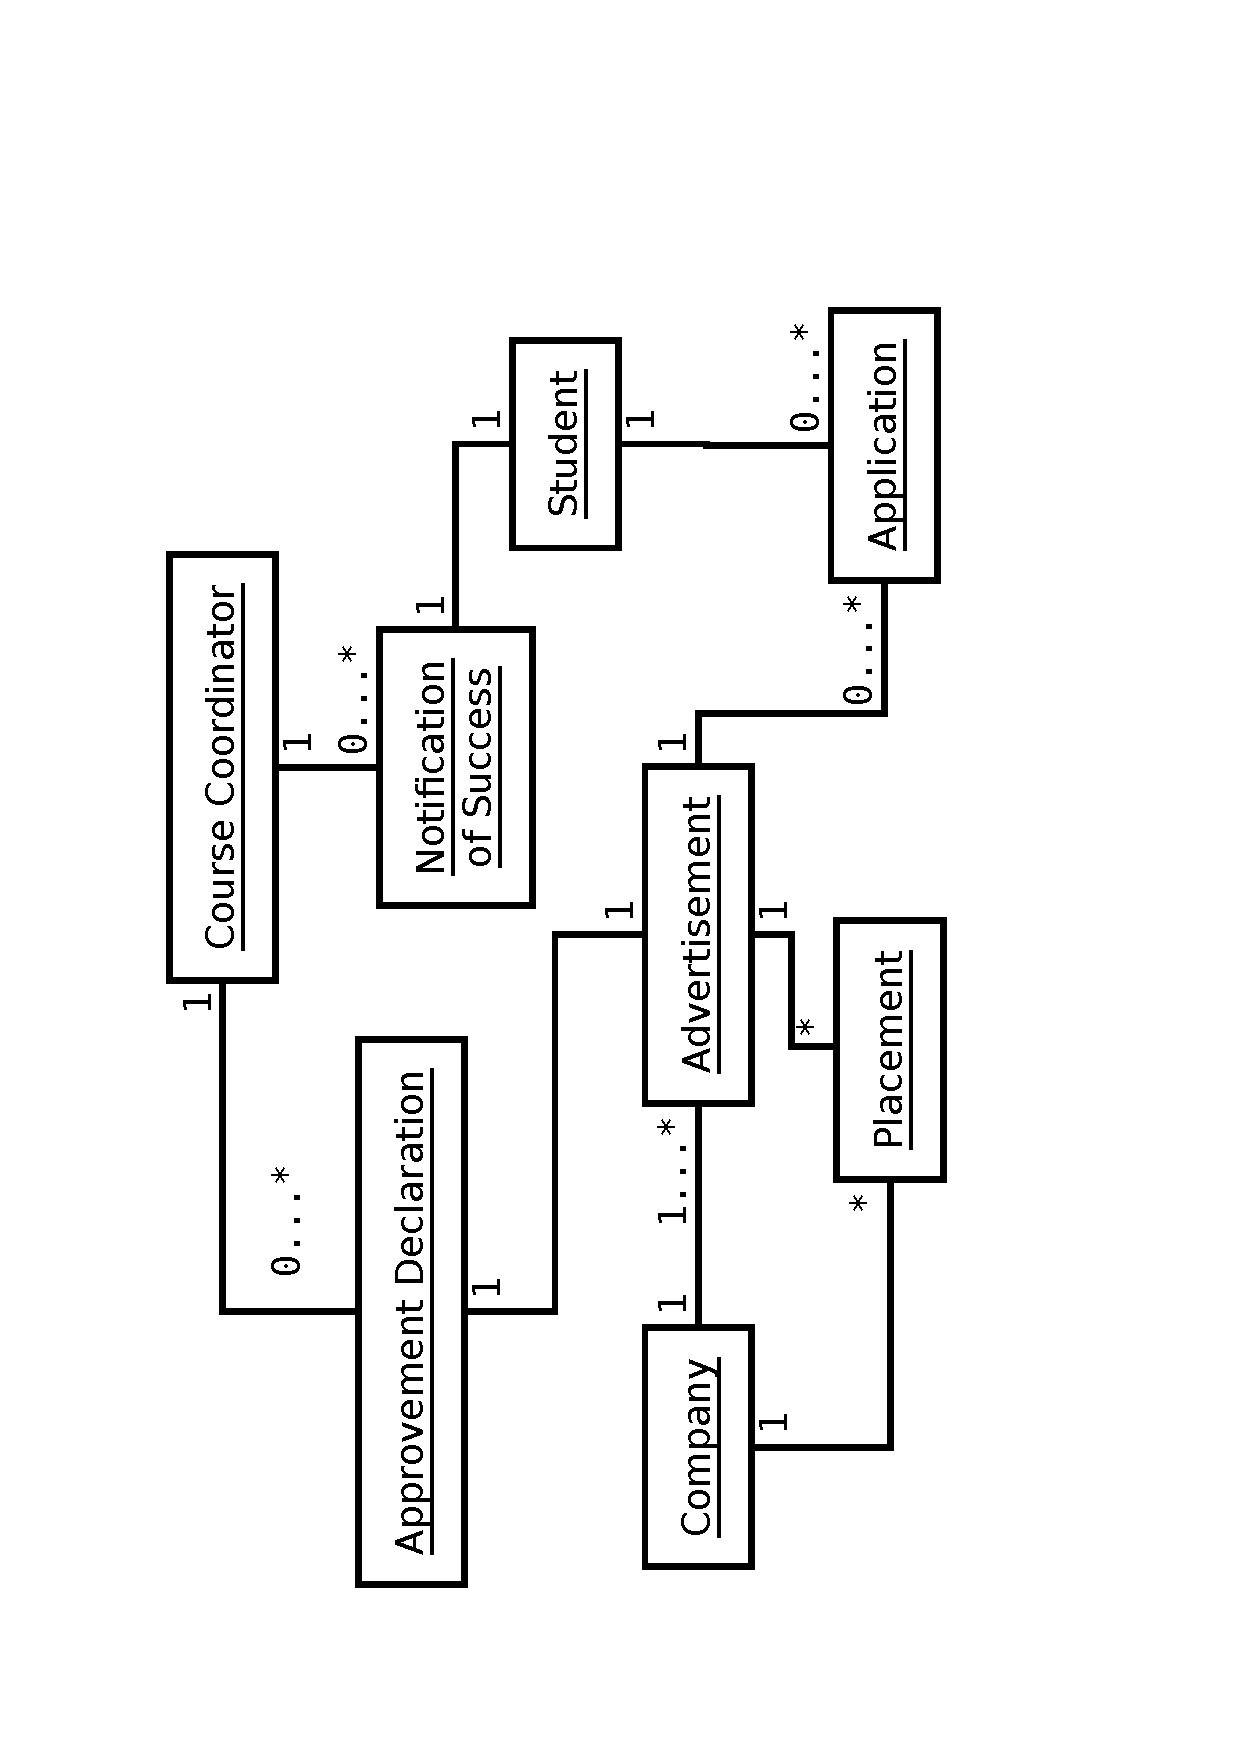
\includegraphics[scale=0.5,angle=-90]{Domain.pdf}
  %\includegraphics[width=60mm]{myfig.png}
  %\includegraphics[height=60mm]{myfig.jpg}
  %\includegraphics[angle=45,width=52mm]{myfig.jpg}

%%%%%%%%%%%%%%%%%%%%%%%%%%%%%%%%%%%%%%%%%%%%%%%%%%%%%%%%%%%%%%%%%%%%%%%%%%%%%%

\section{Use Case Descriptions}
This is a collection of use case descriptions (one per use case).
Think carefully about how to group these descriptions in the document.
You can use the template style provided to format your descriptions:

ADDED THIS TO CHECK


\begin{UseCaseTemplate}
\UseCaseLabel{Student Logs into system}
\UseCaseDescription{A student from the University of Glasgow
  interested in applying for a summer placement/internship gains
  access to the system by logging in.}
\UseCaseRationale{A student should be able to log into the
  system. This gives the system added protection and privacy to those
  who should not have access to the system.}
\UseCasePriority{High}
\UseCaseStatus{Uncomplete}
\UseCaseActors{Student}
\UseCaseExtensions{}
\UseCaseIncludes{}
\UseCaseConditions{}
\UseCaseNonFunctionalRequirements{}
\UseCaseScenarios{Successful log in, Unsuccessful log in.}
\UseCaseRisks{Unable to link with GUID log in which may mean students
  have to enrol for service. }
\UseCaseUserInterface{Log in screen.}
\end{UseCaseTemplate}

\begin{UseCaseTemplate}
\UseCaseLabel{Notification of new placement}
\UseCaseDescription{When a new placement is accepted by the course
  coordinator, all student in Level 3 CS should be notified of it by 
  email.}
\UseCaseRationale{A useful feature to aid CS students in their search
  for a placement}
\UseCasePriority{Medium}
\UseCaseStatus{Uncomplete}
\UseCaseActors{Student, Course Coordinator}
\UseCaseExtensions{}
\UseCaseIncludes{}
\UseCaseConditions{}
\UseCaseNonFunctionalRequirements{}
\UseCaseScenarios{Notification Sent}
\UseCaseRisks{Handeling the response from an email being sent to a 
  non-existent email address or to an email address that causes a 
  bounceback/send fail message. A student neglecting to view emails
  sent by the service due to mass emails sent when many advertisements
  go live on one day.}
\UseCaseUserInterface{Course Coordinator Advert View Screen.}
\end{UseCaseTemplate}

\begin{UseCaseTemplate}
\UseCaseLabel{}
\UseCaseDescription{}
\UseCaseRationale{}
\UseCasePriority{}
\UseCaseStatus{}
\UseCaseActors{}
\UseCaseExtensions{}
\UseCaseIncludes{}
\UseCaseConditions{}
\UseCaseNonFunctionalRequirements{}
\UseCaseScenarios{}
\UseCaseRisks{}
\UseCaseUserInterface{}
\end{UseCaseTemplate}


%%%%%%%%%%%%%%%%%%%%%%%%%%%%%%%%%%%%%%%%%%%%%%%%%%%%%%%%%%%%%%%%%%%%%%%%%%%%%%

\section{Non Functional Requirements}
\begin{itemize}
\item The system can be accessed from anywhere with an internet connection and a
browser. The only authentication required is the staff or student's GUID or 
the company's login.

\item The systems availability should be continual with no unplanned downtime
throughout the time the system should be live. Adding and removing adverts, changing user status,
and any other specific functionality of the system should not require downtime
for the updating of any associated databases. Changes should be instantaneous. There may be maintenance required on
the system to fix any errors but this should be at most one hour per week.

\item Only University of Glasgow students can access the advertisements. This is 
further limited to students registered with the School of Computing Science. 
Companies wishing to submit advertisements are given separate logins at the 
discretion of the Course Coordinator.

\item The mass email system will not impact on the continuing functionality of the 
application and viewing system for the Course Coordinator who should be able 
to complete other tasks while this is in operation.

\item The overall number of concurrent users on the system is dependant on the 
systems infrastructure and should not have a capped user limit.
\end{itemize}

%%%%%%%%%%%%%%%%%%%%%%%%%%%%%%%%%%%%%%%%%%%%%%%%%%%%%%%%%%%%%%%%%%%%%%%%%%%%%%

\section{Summary}

This document, while subject to change if and when requirements change, outlines the functionality and non functional requirements of the Internship Management System to be developed for the University of Glasgow and as defined by requirements gathering by Team W. The system must allow advertisements to be added by a Company and be edited by a Company until being vetted by a Course Coordinator and then can be viewed by a Student. A student must also be able to declare their success in an application to the Course Coordinator through this system.

%%%%%%%%%%%%%%%%%%%%%%%%%%%%%%%%%%%%%%%%%%%%%%%%%%%%%%%%%%%%%%%%%%%%%%%%%%%%%%

\appendix

\section{Glossary}

\begin{itemize}

\item Course coordinator - A member of staff in the University of Glasgow's
School of Computing Science who is the sole administrator for the system and, as
a result, is responsible for reviewing advertisements and keeping track of 
student progress through the system.

\item CS - Computing Science

\item GUID - University of Glasgow user account held by all students and staff
members.

\item ESE - Electronic Software Engineering

\item SE - Software Engineering

\end{itemize}

%\section{Scenarios}

%A collection of scenarios you developed to exercise and refine your
%use cases.

\section{Stakeholder Interview Documentation}

The stakeholder interview conflicted with the requirements specification more
than it clarified. In addition to this, most questions that don't fall into the
former category were typically answered either by stating the specified
feature is out with the scope of the system or the interviewee did not
know the answer.

\section{Stakeholder Panel Documentation}

\begin{itemize}

\item The advertisement submission screen will contain a standard form to
ensure companies submit required information such as duration of placement, and
wages. There will also be a text box to allow a company to submit any other
information they wish to provide.

\item For internships obtained out with the system, the student is to submit
a form to the Course Coordinator. The form is a reduced version of the
aforementioned advertisement submission form.

\item The system will have a single course coordinator whom will act as
the system administrator however this position can be reassigned.

\item An advertisement can be edited by the associated company prior to
publishing.

\item Deletion of advertisements can be executed manually by either the course
coordinator or associated company. This can be done when an internship placement
has been filled up or if a company wishes to amend an advertisement. Amendments
after publication require a deletion of the old advertisement since they are
frozen after publication.

\item University students and staff will use their GUID to login to the system
and companies will use separate accounts supplied by the course coordinator.
Any additional information, such as address and telephone numbers, can then
be obtained via the University's MyCampus system.

\item Via a dashboard, the course coordinator is able to view a summary of
students' statuses in the system. This can be used to contact students not
currently in an application process to remind them to apply to internships. The
course coordinator can download status information to a CSV file.

\item Recruitment agencies and other internship management systems, such as
Club 21, are treated in the same way companies are.

\item The University will already have a mailing list of CS/SE/ESE students
however, the system will not be using this. Instead the system will have its
own mailing list. A student will automatically be added to the mailing list
and can only be removed once a placement has been secured and approved.
Notification of new internships via this mailing list can be sent in a variety
of frequencies, including: instantaneously; daily; bi-weekly etcetera.

\item The stakeholder panel clarified an important point: who can view what
in the system. The course coordinator can be everything. The companies can see
their own advertisements. The students can see all published internships, even
if they have been marked as unsuitable for the student's degree.

\end{itemize}

%%%%%%%%%%%%%%%%%%%%%%%%%%%%%%%%%%%%%%%%%%%%%%%%%%%%%%%%%%%%%%%%%%%%%%%%%%%%%%

\end{document}

%%%%%%%%%%%%%%%%%%%%%%%%%%%%%%%%%%%%%%%%%%%%%%%%%%%%%%%%%%%%%%%%%%%%%%%%%%%%%%
